
\documentclass{article}
\usepackage[utf8]{inputenc}
\usepackage{authblk}
\usepackage{setspace}
\usepackage[margin=1.25in]{geometry}
\usepackage{graphicx}
%\graphicspath{ {images/} }
\graphicspath{ {./images/} }
\usepackage{caption}
\usepackage{subcaption}
\usepackage{amsmath}
\usepackage{lineno}
\usepackage{listings}
%\usepackage[english]{babel}
%\usepackage{biblatex}
%\usepackage{cite}
%\usepackage{biblatex}
%\linenumbers

%%%%%% Bibliography %%%%%%
% Replace "sample" in the \addbibresource line below with the name of your .bib file.
\usepackage[style=ieee, 
citestyle=numeric-comp,
sorting=none]{biblatex}
\addbibresource{mybib1.bib}

%%%%%% Title %%%%%%
% Full titles can be a maximum of 200 characters, including spaces. 
% Title Format: Use title case, capitalizing the first letter of each word, except for certain small words, such as articles and short prepositions
\title{Empirical power calculation and Resampling techniques}

%%%%%% Authors %%%%%%
% Authors should be listed in order of contribution to the paper, by first name, then middle initial (if any), followed by last name.
% Authors should be listed in the order in which they will appear in the published version if the manuscript is accepted. 
% Use an asterisk (*) to identify the corresponding author, and be sure to include that person’s e-mail address. Use symbols (in this order: †, ‡, §, ||, ¶, #, ††, ‡‡, etc.) for author notes, such as present addresses, “These authors contributed equally to this work” notations, and similar information.
% You can include group authors, but please include a list of the actual authors (the group members) in the Supplementary Materials.
%\author[1*$\dag$]{Kalyango Jovan}
%\author[2$\dag$]{Author Two}
\author{Kalyango Jovan}
%\author[1,2]{Author Four}

%%%%%% Affiliations %%%%%%
\affil[1]{UMC, Utrecht University, Utrecht, The Netherlands.}
\affil[2]{Department of Methodology and Statistics, Utrecht University, Utrecht, The Netherlands.}
\affil[*]{Corresponding author. Email:j.kalyango@uu.nl}
%\affil[$\dag$]{These authors contributed equally to this work.}

%%%%%% Date %%%%%%
% Date is optional
\date{}

%%%%%% Spacing %%%%%%
% Use paragraph spacing of 1.5 or 2 (for double spacing, use command \doublespacing)
\doublespacing

\begin{document}

\maketitle

%%%%%% Abstract %%%%%%
\begin{abstract}
Power calculations ans sample size are an important part of designing new sequence-based association studies.It is desirable to develop methods that can quickly and accurately compute power without intensive Monte Carlo simulations but in  this article we are comparing the R in built function and the function that is manually built.In our resampling procedures, a statistic of interest is calculated from multiple samples.Permutation reshuffles the observed cases, sampling without replacement.Bootstrapping selects from the populations of observed cases, sampling with replacement.Monte Carlo typically samples with replacement from theoretical distributions with specific characteristics. A large number of resamples (say 10,000+) is desirable to give stable results.

\begin{itemize}
    \item Empirical power calculation\
    \item Resampling techniques\
\end{itemize} 
\end{abstract}

%%%%%% Equations %%%%%%
\subsection*{Equations}


\medskip we are supposed to use Equation \ref{eq:1} to create a function that computes the t-test. The formula for the t-test is as follows,  where Equation \ref{eq:2} is ,Equation \ref{eq:3} and Equation \ref{eq:4} below.
\begin{equation} \label{eq:1}
t =\frac{({y1bar}-{y2bar})}{s*\sqrt(1/n1+1/n2)}
\end{equation}
where n1 and n2 are the two sample sizes, y1bar and y2bar are the two sample means, and s is the square root of the pooled estimate of the variance, \begin{equation*} s^2\end{equation*} which is equal to:
\begin{equation} \label{eq:2}
\begin{split}
s^2 & = \frac{(n1- 1)s1^2 + (n2- 1)s2^2}{(n1-1)+ (n2-1)} \\
\end{split}
\end{equation}
Make a function to compute the t-test with the aforementioned formulas and which starts as follows:
\begin{equation} \label{eq:3}
\begin{split}
\hat{\beta}& =(X'X)^-1*(X'y)\\
\end{split}
\end{equation}
\begin{equation} \label{eq:4}
\begin{split}
\hat{y}& = X\beta\\
\end{split}
\end{equation}


%%%%%% Figures and Tables %%%%%%
\subsection*{Figures and Tables}
 To test the function I built, I will use the data which obtained from a study by air force psychologists conducting research into the relative effectiveness of training pilots as seen in \textbf{Table 1}. The first training method consists of computer simulated flight instruction (CSFI) while the second training method uses traditional flight instruction (TFI). The 18 pilots were randomly assigned to the two experimental conditions CSFI and TFI and the performance test scores in each condition are displayed in \textbf{Table 1}. Then will calculate the t-statistic with the newly created function and check the results by analyzing the same data with the in-built R function t.test and compare the results.
\begin{table}[!h]
    \caption{Flight instruction data}    
    \centering
    \begin{tabular}{cc}
            \hline
            CSFI & TFI\\  
            \hline
            2 & 1 \\ 
            5 & 1 \\
            5 & 2 \\ 
            6 & 3 \\
            6 & 3 \\ 
            7 & 4 \\
            8 & 5 \\ 
            9 & 7 \\
              & 7 \\ 
              & 8 \\
            \hline
            \end{tabular}
    \label{tab:1}
\end{table}
\textbf{Figure 1} is a plot of fitted values vs residuals is the inverted(reversed) plot of "plot(model,which = 1)", and since the plot is inverted( residuals vs fitted ) shows no clear linear relationship also the plot(fitted vs residuals) display no clear linear relationship between the predicted values and residuals, but we can notice some outliers instead.
\begin{figure}
 \centering
  \begin{subfigure}[b]{0.5\textwidth}
      \centering
        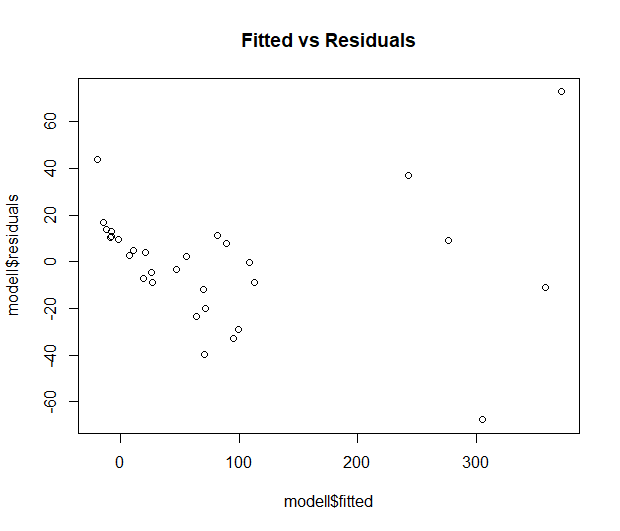
\includegraphics[width=0.8\textwidth]{Rplotf.png}
       \caption{Fitted values vs Residuals}
       \label{fig.1}
 \end{subfigure}
 \begin{subfigure}[b]{0.5\textwidth}
      \centering
      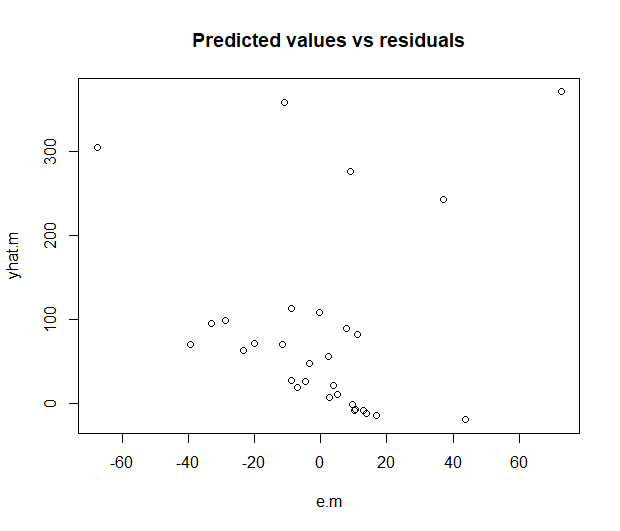
\includegraphics[width=0.8\textwidth]{Rplotp.png}
      \caption{Predicted values vs Residuals}
      \label{fig.2}
 \end{subfigure}

\end{figure}

%%%%%% Main Text %%%%%%


\section{Introduction}
A t test is a type of statistical test that is used to compare the means of two groups. It is one of the most widely used statistical hypothesis tests in range of studies\cite{davison2002introduction}. There are two types of statistical inference: parametric and nonparametric methods. Parametric methods refer to a statistical technique in which one defines the probability distribution of probability variables and makes inferences about the parameters of the distribution\cite{pmid28898401}.In cases in which the probability distribution cannot be defined, nonparametric methods are employed. T tests are a type of parametric method; they can be used when the samples satisfy the conditions of normality, equal variance, and independence.
T tests can be divided into two types. There is the independent t test, which can be used when the two groups under comparison are independent of each other, and the paired t test, which can be used when the two groups under comparison are dependent on each other. T tests are usually used in cases where the experimental subjects are divided into two independent groups, with one group treated with A and the other group treated with B. Researchers can acquire two types of results for each group (i.e., CSFI and TFI). An independent t test can be used for an intergroup comparison between two groups.Sample size and power calculations are an important part of designing new sequence-based association studies.

Resampling methods have become practical with the general availability of cheap rapid
computing and new software Compared to standard methods of statistical inference, these
modern methods often are simpler and more accurate, require fewer assumptions, and have
greater generalizability. Resampling provides especially clear advantages when assumptions of
traditional parametric tests are not met, as with small samples from non-normal distributions.
Additionally, resampling can address questions that cannot be answered with traditional
parametric or nonparametric methods, such as comparisons of medians or ratios. The resampling
methods for testing means, medians, ratios, or other parameters are the same, so we do not need
new methods for these different applications. Thus, resampling also has advantages of
conceptual simplicity.
Parametric tests can be criticized because they require restrictive assumptions, tests may be
difficult to interpret, and no tests are readily available for some interesting statistics. More
importantly, parametric tests can fail to detect important effects or give misleading results under
some conditions. For example, adding a relatively extreme observation can reduce the sensitivity
of a parametric test, even if the observation is in the direction of observed effects. 
Three resampling methods that are commonly used for different purposes:
Permutation methods use sampling without replacement to test hypotheses of no effect‟;
Bootstrap methods use sampling with replacement to establish confidence intervals;
Monte Carlo methods use repeated sampling from populations with known characteristics to
determine how sensitive statistical procedures are to those characteristics.

\section{Methods}
You have the following data: two groups, an experimental and a control group, of 50 participants each, that were randomly assigned to two conditions. The values of interest are the test scores on an exam for both groups. The participants in the experimental grouped received a special training on learning strategies prior to an exam. Based on past research you expect that the control group will have a mean of 150 on the test with standard deviation of 15 and that the experimental group will have a mean on the test scores that is 10 points higher than the control group, with the same standard deviation. We perform a t-test on the data and we are interested to know the power of the test. We will estimate the power in two ways, using the in-built R function power.t.test and by simulation.By assuming that the data are approximately normal, simulate one sample of data and perform a t-test using the R in-built t-test function. Then,we will approximate the power by simulation. We still continue to maintain that the data are normally distributed, then we write a function that generates data and performs a t-test 1000 times and that stores the values of the t-statistic (or the p-value) in a vector. Thinking about the definition of power in terms of rejecting the null hypothesis, we obtain an estimate of the power in this new situation and compare the results with those given by power.t.test. 
Furthermore,we choose an appropriate resampling technique and make a function that performs a hypothesis test based on the t-statistic produced by the standard t-test function, the in-built sample() function to perform the resampling of the data. we include relevant statistics in the function and give the function a clear structure ( by choosing a sensible input arguments, organize the output in an efficient way, as explained in discussion, results and conclusion). The results of the resampling technique used on the Flight instruction data. we program the drawing of random samples when we do not want to use the sample() function, we then modify the function we have programmed in earlier in such a way that it does not use the sample() function anymore (so we will have to work with indices). Run your new function and show that we can obtain the same results as in we first programmed. 
We have to choose the best resampling technique(s) to use, if we would be interested in estimation instead of hypothesis testing, we make an R function that performs resampling for estimation purposes using the mean difference between two groups from the t-test function. The function is producing all relevant aspects of estimation, as stated and discussed in the discussion section, these aspects and put them in perspective. Still we use the Flight instruction data to show the results of the function.


\subsection{Statistical Analysis}
We begin our analysis by  set seed to get stable results, set.seed(13) , for replication purposes,  Make two groups, group 1 with mean=150 and sd=15 and group 2 with mean=10 and sd=15, we then use, t.test(group1, group2)  and  finally,to get a power estimate, given by R
power.t.test(n = 50, delta = 10, sig.level = .05, sd = 15, type = "two.sample", alternative = "two.sided") to respond to the first aim of this article. We write the function, with input parameters; n1, n2, mean1, mean2, sd1, sd2, times. Inside the function we first make vectors to store results, make names for the columns to extract them later,the loop in the function, has sample the two groups: can give n, mean and sd in the function to make it useful for multiple usage. Compute t-tests and store its results in the matrix, we finally test the function: 
my.boot.t.test(n1 = 50, n2 = 50, mean1 = 150, mean2 = 160, sd1 = 15, sd2 = 15, times = 1000). 
We made a function for a resample-test that can do both bootstrap and permutation test. We would normally use the bootstrap, because then there are more possible samples and this function can be used for smaller groups as well.
Function for resample t-test: sided.test is either '1' or '2', default '1'. For sampling.method, choose between 'bootstrap' or 'permutation.test': bootstrap default. 
For estimation we would choose for the bootstrap resampling method. We would choose for this because this method would work with really small samples where the permutationtest wouldn't work because of too few possible permutations. Also, the bootstrap deals better with differences in variance when estimating, which is often the case for a t-test. We write a function: bootstrap for estimation purposes.




\section{Results}

On this seed, a p-value of .00238 is obtained, what means that the group difference is significant. However, since this is only one simulation, we can not be too sure about this outcome, because every simulation can get other results. To get a more robust conclusion, we should perform far more simulations before we can conclude anything.
If power is seen as the percentage of simulations that find a significant result, we get a power estimate of .916. When the power of the test is evaluated with the R-function, we obtain a power of .910. These values differ a little bit, but are more or less of the same magnitude. However, when more simulations are used for the bootstrap, the power estimate approaches the in-build power estimate more (10.000 simulations: power estimate = .908, 100.000 simulations: power estimate = .910). So with enough simulations, we will probably find the power estimate R has given in the supplementary materials.
 The obtained results differ a little bit from the last question. This is because now, we take pseudo-random numbers for the indices, which still has randomness and therefore isn't exactly the same as question 1. Even with the same seed, we get a different result, since we sample indices now. However, the number of samples we took was not that high. When we take more samples (for example 100,000) the p-values are almost the same (both .105). We looked really hard for a way to get samples without even taking random indices. However, then your simulation would end up with systematic samples, what is not the goal of a simulation. A possible way to 'sample' without randomness, is by taking every possible permutation. However, then the number of simulations would be enormous and when only taking 1000, the systematic approach in permutating doesn't have the character of a good simulation.
 Our estimate showed that the true mean difference of this population lays with 0.95 certainty in the confidence interval of 0.15 and 3.85125. This confidence interval is computed with the percentile method. The computed bias shows how much our mean estimate differs from the true observed mean difference. Bias has to be as low as possible, ideally even 0. The more bootstrap samples used, the smaller the bias will get. N = 1000, as used in our example, is quite high and therefore, the estimation has quite low bias. The computed standard error of the sampling distribution tells something about how spread the data is. When using a high number of bootstrap samples, 2 standard errors below and above the mean will be the same as the obtained values of the 0.95-percentile confidence interval. This is the case with our output as well.



\section{Discussion}



\section*{Supplementary Materials}
The documentation of this project, including the R code and instructions to reproduce the results,
is available in the research repository at https://github.com/KalyangoJovan/Research-Repository.



 
\section{Referenses} 
\printbibliography






\end{document}
